\section{Missing Proofs}
\label{sec:appendix}

\begin{lemma}
Consider a hypergraph $\mH = (\mV, \mE)$ with valuations $\{v_e\}_{e \in \mE}$. Then, there exists a uniform bundle price $p^{b}$ that achieves revenue $O(\log m)$ away from  $\sum_{e \in \mE} v_e$, where $m = |\mE|$.
\end{lemma}

\begin{proof}
Consider the valuations $v_{e_1}, v_{e_2}, \dots, v_{e_m}$ in increasing order. We claim that setting $p^{b}(e)  = v_{e_j}$ for very $e \in \mE$ achieves the 
desired approximation for some edge $e_{j}$. 
The revenue $R_j$ we obtain by selling at price $v_{e_j}$ is $R_j \geq (m-j+1)v_{e_j} $. Then, the best revenue $R$ has $R \geq R_j$.
%Then $m v_{e_1} < \textsf{OPT}/ \log m$ since we can sell each edge if the bundle price is the smallest valuation. Similarly, $(m - i) v_{e_i} < \textsf{OPT}/ \log m$ for each edge.
Adding up all inequalities, we get:
	
	\begin{equation*}
	\begin{aligned}
	\sum_{j=1}^m v_{e_j} \leq  \sum_{j=1}^m \frac{R_j}{m-j+1} \leq R \sum_{j=1}^m \frac{1}{j} = R \cdot O(\log m) .
	\end{aligned}
	\end{equation*}
\end{proof}


\begin{lemma} \label{lem:lb1}
There exists a hypergraph $\mH = (\mV, \mE)$ with additive valuations, such that any uniform bundle price produces revenue $\Omega(\log m)$ from the optimal revenue
$\sum_{e \in \mE} v_e$.
\end{lemma}	

\begin{proof}
	Consider $n$ items and $m$ buyers ($n=m$), such that buyer $b_i$ wants item $i$ for price $1/i$. It is easy to see that the valuations are additive, and that the optimal revenue
	is $\sum_i 1/i = \Theta(\log m)$. Consider a uniform bundle price where $p^b(e) = 1/c$ for some $1 \leq c \leq m$. Then, the seller can sell edges that have valuation at least $1/c$. Observe that the number of such edges is at most $c$. Therefore, the revenue can be at most $\sum_{e:v_e \leq 1/c} 1/c = O(1)$.
\end{proof}

\begin{lemma} \label{lem:lb2}
There exists a hypergraph $\mH = (\mV, \mE)$ with uniform valuations, such that any item pricing solution produces revenue $\Omega(\log m)$ from the optimal revenue
$\sum_{e \in \mE} v_e$.
\end{lemma}
\begin{proof}
	Let $\mC_i$ denote the class of customers that desire exactly $i $ items. We construct the hypergraph instance as follows: Each class of customers $\mC_i$ has 
	exactly size $\lceil n/i \rceil$ and each customer in $\mC_i$ is assigned a partition of $i$ items such that no two customers share any item. Thus, the total number of hyperedges is $m = \sum_{i} \vert \mC_i \vert = \Theta( n \log n)$. Figure~\ref{fig:laminar} shows  an instance for $n=6$. We fix the valuation $v_e = 1$ for all hyperedges. Selling each edge at price $p^{b}(e) = 1$, we extract the full revenue of $\Theta(n \log n)$.
	
	Next, we show that no item pricing solution can do better than $O(n)$. We will show this by induction on the customer class $\mC_i$. The base case is revenue obtained by selling edges to customers in $\mC_1$. Since there are at most $n$ edges, the maximum revenue is $O(n)$. Consider the customer class $\mC_k$. Let denote $0 < \alpha \leq 1$ be the fraction of edges sold to customers in $\mC_k$ and let $\mE_k$ denote such edges. Then, the maximum revenue that can be extracted is $\alpha \lceil n/k \rceil$. We distinguish three types of edges: $(i)$ edges that share at least one item with edges in $\mE_k$ $(ii)$ edges that do not share any item with edges in $\mE_k$ $(iii)$ edges that are strictly contained within $\mE_k$. By the induction hypothesis, the maximum revenue that can be extracted from all type $(ii)$ edges is at most $O(n)$. Each edge in $\mE_k$ can overlap with at most $2(k-1)$ edges that have size strictly lesser than $k$. Thus, the revenue extracted from type $(i)$ edges is at most $2(k-1) \alpha \lceil n/k \rceil = O(n)$. Consider an edge $e' \in \mE_k$ and let $w_1, \dots w_k$ be the weights of items in $e'$. Since the seller is able to sell $e'$, we have that $w_1 + \dots w_k \leq 1$. Observe that the maximum revenue of all edges of size strictly lesser than $k$ (say $k'$) using items in $e'$ is also at most $w_1 + \dots w_k \leq 1$ which gives revenue of $O(k)$. 
\end{proof}




\begin{lemma} \label{lem:lb3}
There exists a hypergraph $\mH = (\mV, \mE)$ with submodular valuations, such that any uniform bundle pricing and any item pricing produces revenue $\Omega(\log m)$ from the optimal revenue
$\sum_{e \in \mE} v_e$.
\end{lemma}	


\begin{figure}[t]
	\scalebox{1}{
		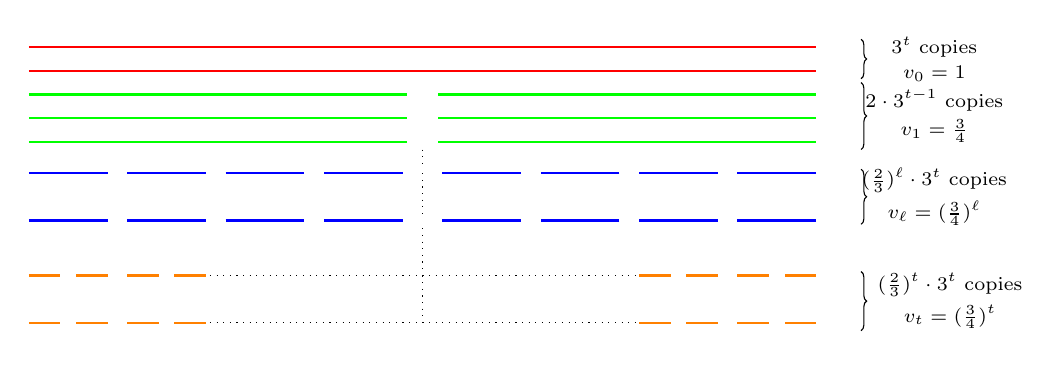
\begin{tikzpicture}
			\draw [red, thick] (-5,5) to (5,5);
			\draw [red, thick] (-5,4.7) to (5,4.7);
			
			\draw [decorate,decoration={brace,amplitude=2pt,raise=2pt},yshift=0pt]
			(5.5,5.1) -- (5.5,4.6) node [black,midway,xshift=1cm] {
				\shortstack{ \scriptsize $3^t$ copies \\ \scriptsize $v_0 = 1$}};
			
			\draw [green, thick] (-5,4.4) to (-0.2,4.4);
			\draw [green, thick] (0.2,4.4) to (5,4.4);
			
			\draw [green, thick] (-5,4.1) to (-0.2,4.1);
			\draw [green, thick] (0.2,4.1) to (5,4.1);			
			
			\draw [green, thick] (-5,3.8) to (-0.2,3.8);
			\draw [green, thick] (0.2,3.8) to (5,3.8);			
			
			\draw [decorate,decoration={brace,amplitude=2pt,raise=2pt},yshift=0pt]
			(5.5,4.55) -- (5.5,3.7) node [black,midway,xshift=1cm] {
			\shortstack{ \scriptsize $2 \cdot 3^{t-1}$ copies \\ \scriptsize $v_1 = \frac{3}{4}$}};			
		
			\draw[dotted]  (0, 3.7) -- (0, 3.45);
			
			\draw [blue, thick] (-5,3.4) to (-4,3.4);
			\draw [blue, thick] (-3.75,3.4) to (-2.75,3.4);			
			\draw [blue, thick] (-2.5,3.4) to (-1.5,3.4);			
			\draw [blue, thick] (-1.25,3.4) to (-0.25,3.4);									
			\draw [blue, thick] (5,3.4) to (4,3.4);
			\draw [blue, thick] (3.75,3.4) to (2.75,3.4);			
			\draw [blue, thick] (2.5,3.4) to (1.5,3.4);			
			\draw [blue, thick] (1.25,3.4) to (0.25,3.4);			
			
			\draw[dotted]  (0, 3.4) -- (0, 2.85);
			
			\draw [blue, thick] (-5,2.8) to (-4,2.8);
			\draw [blue, thick] (-3.75,2.8) to (-2.75,2.8);			
			\draw [blue, thick] (-2.5,2.8) to (-1.5,2.8);			
			\draw [blue, thick] (-1.25,2.8) to (-0.25,2.8);									
			\draw [blue, thick] (5,2.8) to (4,2.8);
			\draw [blue, thick] (3.75,2.8) to (2.75,2.8);			
			\draw [blue, thick] (2.5,2.8) to (1.5,2.8);			
			\draw [blue, thick] (1.25,2.8) to (0.25,2.8);
			
			\draw [decorate,decoration={brace,amplitude=2pt,raise=2pt},yshift=0pt]
			(5.5,3.45) -- (5.5,2.75) node [black,midway,xshift=1cm] {
				\shortstack{ \scriptsize $(\frac{2}{3})^\ell \cdot 3^{t}$ copies \\ \scriptsize $v_\ell = (\frac{3}{4})^{\ell}$}};			
			
			\draw[dotted]  (0, 2.7) -- (0, 2.1);
			
			\draw [orange, thick] (-5,2.1) to (-4.6,2.1);
			\draw [orange, thick] (-4.4,2.1) to (-4,2.1);
			\draw [orange, thick] (-3.75,2.1) to (-3.35,2.1);
			\draw [orange, thick] (-3.15,2.1) to (-2.75,2.1);			
			\draw[dotted] (-2.7, 2.1) to (2.7, 2.1)			;
			\draw [orange, thick] (5,2.1) to (4.6,2.1);
			\draw [orange, thick] (4.4,2.1) to (4,2.1);
			\draw [orange, thick] (3.75,2.1) to (3.35,2.1);
			\draw [orange, thick] (3.15,2.1) to (2.75,2.1);			
			
			
			\draw[dotted]  (0, 2.1) -- (0, 1.5);
			
			\draw [orange, thick] (-5,1.5) to (-4.6,1.5);
			\draw [orange, thick] (-4.4,1.5) to (-4,1.5);
			\draw [orange, thick] (-3.75,1.5) to (-3.35,1.5);
			\draw [orange, thick] (-3.15,1.5) to (-2.75,1.5);			
			\draw[dotted] (-2.7, 1.5) to (2.7, 1.5)			;
			\draw [orange, thick] (5,1.5) to (4.6,1.5);
			\draw [orange, thick] (4.4,1.5) to (4,1.5);
			\draw [orange, thick] (3.75,1.5) to (3.35,1.5);
			\draw [orange, thick] (3.15,1.5) to (2.75,1.5);			
			
			\draw [decorate,decoration={brace,amplitude=2pt,raise=2pt},yshift=0pt]
			(5.5,2.15) -- (5.5,1.4) node [black,midway,xshift=1.2cm] {
				\shortstack{ \scriptsize $(\frac{2}{3})^{t} \cdot 3^{t}$ copies \\ \scriptsize $v_{t} = (\frac{3}{4})^{t}$}};			
			
			
		\end{tikzpicture}
	}
	\caption{Laminar family construction for the lower bound of Lemma~\ref{lem:lb3}.}
	\label{fig:laminar}
\end{figure}

\begin{proof}

We construct a laminar family of sets arranged in binary tree fashion as follows: The root node is the set of all $n = 2^{t}$ items. At depth $\ell$, there are $2^\ell$ sets, each of size $\left( \frac{n}{2^{\ell}} \right)$ formed by partitioning each set at depth $\ell-1$ of size $\left( \frac{n}{2^{\ell - 1}} \right)$ into two. Further, each set $S$ at depth $\ell$ has valuation $v(S) = \left( \frac{3}{4} \right)^{\ell}$ and $c_\ell = \left( \frac{2}{3} \right)^{\ell} 3^t$ copies of itself. Figure~\ref{fig:laminar} shows the construction. Let $\mL$ denote the family of laminar sets in the construction. Although $v$ is only defined on $\mL$, it can be extended to any set $A\subseteq V$ by defining $v(A) = \min_{X \subseteq \mL} \sum_{S \in X} v(S)$ where $X$ is a set cover of $A$. Note that $v(A)$ is monotone and subadditive. We first prove that $v(A)$ is actually submodular.

Let us introduce some more notations. Let $\bA$ denote the minimum weighted set covering of a set $A$, i.e. $\bA = \argmin_{X \subseteq \mL} \sum_{S \in X} v(S)$  where $X$ is a set cover of $A$. We overload the valuation function $v$ to mean $v(\bA) = \sum_{S \in \bA} v(S)$ and define $A^{*} = \bigcup_{X \in \bA} X$ to be the set of items covered by some set in $X$. For any two sets $A, B \in 2^{[n]}$, it holds that $v(A) + v(B) = v(\bA) + v(\bB)$ by definition of valuation function. Observe that $A \cap B \subseteq A^{*} \cap B^{*}$ and by monotonicity, we have $v(A \cap B) \leq v(A^{*} \cap B^{*})$. Similarly, $v(A \cup B) \leq v(A^{*} \cup B^{*})$. Thus, to show submodularity, it suffices to verify that 
\begin{equation}\label{eqnsubmodular}
v(\bA) + v(\bB) \geq v(A^{*} \cup B^{*}) + v(A^{*} \cap B^{*}).
\end{equation}
Assume that the largest set in $\bA\cup \bB$ has size $2^u$. We verify (\ref{eqnsubmodular}) by applying induction to $u$.

\smallskip
\introparagraph{Base Case} If $u=0$, i.e. $\bA$ and $\bB$ only contain sets with size 1, let $L^{0}_1, \dots, L^{0}_{n} \in \mL$ denote all singleton sets. Define for each $i$ $A_i = A^* \cap L^{0}_i, B_i = B^* \cap L^{0}_i$. Then
\begin{eqnarray*}
	& &v(\bA) + v(\bB) \\
	&=& v(A_1) + \dots + v(A_n) +  v(B_1) + \dots + v(B_n) \\
	& = & v(A_1) + v(B_1) + \dots + v(A_n) + v(B_n) \\
	& = & v(A_1 \cap B_1) + \dots + v(A_n \cap B_n) + v(A_1 \cup B_1) + \dots + v(A_n \cup B_n) \\
	& = & v((A^* \cap B^*) \cap L^{0}_1) + \dots + v( (A^* \cap B^*) \cap L^{0}_n) +  v( (A^* \cup B^*) \cap L^{0}_1) + \dots + v( (A^* \cup B^*) \cap L^{0}_n) \\
	& \geq & v(A^{*} \cup B^{*}) + v(A^{*} \cap B^{*}).
\end{eqnarray*}
Here the first equality holds since $v(\bA)$ and $v(\bB)$ are defined only by sets with size 1.
The third equality holds since each $\bA_i$ and $\bB_i$ is either an empty set or singleton. The fourth equality holds by definition of $A_i$ and $B_i$. The fifth inequality holds by subadditivity of $v$.

\smallskip
\introparagraph{Inductive Case} Assume that $v(\bA) + v(\bB) \geq v(A^{*} \cup B^{*}) + v(A^{*} \cap B^{*})$ holds if all sets in $\bA\cup \bB$ have size at most $2^{u-1}$. Consider all sets of size $2^u$: $L^{u}_1, \dots, L^{u}_{n/2^u} \in \mL$ and define for every $i$ $A_i = A^* \cap L^{u}_i, B_i = B^* \cap L^{u}_i$. Using the same argument as in the base case, we have 

\begin{eqnarray*}
& &v(\bA) + v(\bB)\\
& = &v(A_1) + \dots + v(A_{n/2^{u}}) +  v(B_1) + \dots + v(B_{n/2^{u}})\\
& =  & v(A_1) + v(B_1) + \dots + v(A_{n/2^{u}}) + v(B_{n/2^{u}}) \\
& \geq & v(A_1 \cap B_1) + \dots + v(A_{n/2^{u}} \cap B_{n/2^{u}}) + v(A_1 \cup B_1) + \dots + v(A_{n/2^{u}} \cup B_{n/2^{u}}) \\
& = & v( (A^* \cap B^*) \cap L^{u}_1) + \dots + v( (A^* \cap B^*) \cap L^{u}_{n/2^{u}}) +  v( (A^* \cup B^*) \cap L^{u}_1) + \dots + v( (A^* \cup B^*) \cap L^{u}_{n/2^{u}}) \\
&\geq &v(A^{*} \cup B^{*}) + v(A^{*} \cap B^{*}).
\end{eqnarray*}

Here the third inequality is where we invoke the inductive hypothesis: if $v(A_i)=v(L_i^u)$ or $v(B_i)=v(L_i^u)$, then $v(A_i)+v(B_i)=v(A_i\cup B_i)+v(A_i\cap B_i)$. Otherwise, $v(A_i)$ and $v(B_i)$ are both defined by sets with size at most $2^{u-1}$, by inductive hypothesis $v(A_i)+v(B_i)\geq v(A_i\cup B_i)+v(A_i\cap B_i)$. Thus (\ref{eqnsubmodular}) always holds, which means $v$ is indeed a submodular function.

If we price every bundle at its value, the revenue extracted is maximized. For each level $\ell$, there are $2^{\ell}$ sets and $(2/3)^{\ell} \cdot 3^{t}$ copies of each set. Thus, the total revenue from all $t+1$ levels is
\begin{align*}
	\textsf{OPT} = \sum_{\ell = 0}^{t} v_\ell c_\ell 2^\ell = (t+1)\left( \frac{3}{4} \right)^{\ell}  \cdot \left( \frac{4}{3} \right)^{\ell} \cdot  3^{t} = (t+1) \cdot 3^{t}.
\end{align*}

%However, it remains to be shown that the third inequality is true, i.e. $v(\bA_i) + v(\bB_i) \geq v(\bA_i \cup \bB_i) + v(\bA_i \cap \bB_i)$. If either $\bA_i = L^{u}_i$ or $\bB_i = L^{u}_i$, then the inequality (equality in this case) holds.

%Otherwise, if each $\bA_i$ and $\bB_i$ is empty, it means that $\bA_i$ and $\bB_i$ are covered by sets with height $< u$. Define $\bA'_i = \bA_i \cap L^{u-1}_i, \bB'_i = \bB_i \cap L^{u-1}_i$. By the inductive hypothesis, it holds that $v(\bA'_i) + v(\bB'_i) \geq v(\bA'_i \cup \bB'_i) + v(\bA'_i \cap \bB'_i)$ and thus,

%\begin{align*}
%	v(\bA_i) + v(\bB_i) & = v(\bA'_1) + \dots + v(\bA'_{n/2^{u-1}}) +  v(\bB'_1) + \dots + v(\bB'_{n/2^{u-1}}) \displaybreak[0]\\
%	& = v(\bA'_1) + v(\bB'_1) + \dots + v(\bA'_{n/2^{u-1}}) + v(\bB'_{n/2^{u-1}}) \displaybreak[0] \\
%	& \geq v(\bA'_1 \cap \bB'_1) + \dots + v(\bA'_{n/2^{u-1}} \cap \bB'_{n/2^{u-1}}) + v(\bA'_1 \cup \bB'_1) + \dots + v(\bA'_{n/2^{u-1}} \cup \bB'_{n/2^{u-1}}) \displaybreak[0]\\
%	& = v( (\bA_i \cap \bB_i) \cap L^{u-1}_1) + \dots + v( (\bA_i \cap \bB_i) \cap L^{u-1}_{n/2^{u-1}}) +  v( (\bA_i \cup \bB_i) \cap L^{u-1}_1) + \dots + v( (\bA_i \cup \bB_i) \cap L^{u-1}_{n/2^{u-1}}) \displaybreak[0]\\
%	& \geq v(\bA_i \cup \bB_i) + v(\bA_i \cap \bB_i)	
%\end{align*}

Next, we will show that no uniform bundle pricing or item pricing can extract revenue more than $O(3^{t})$.

For optimal bundle pricing, the first observation is that we need to consider only bundle prices of the form $\left( \frac{3}{4} \right)^{k}$, i.e. the value of some set in the laminar system. Let the bundle price chosen be $\left(\frac{3}{4} \right)^{k}$, then we can sell all edges at depth $\leq k$. The revenue collected by such bundle pricing is 
\begin{equation*}
\textsf{OPT}_B = \sum_{i \leq k} \left( \frac{3}{4} \right)^{k} \cdot \left( \frac{2}{3} \right)^{i} \cdot 3^{t} \cdot 2^{i} 
 = \left( \frac{3}{4} \right)^{k} \cdot 3^{t} \sum_{i \leq k} \left( \frac{4}{3} \right)^{i} \displaybreak[0]\\
 \leq \left( \frac{3}{4} \right)^{k} \cdot 3^{t+1} \cdot \left( \frac{4}{3} \right)^{k} = O(3^{t}).
\end{equation*}

For optimal item pricing, let $k$ be the smallest depth for any set sold by an optimal item pricing solution. By symmetry we can assume that all sets with depth $k$ are sold. Then the sum of prices of all items is upper bounded by $\sum_{i}p_i\leq (\frac{3}{4})^{k}\cdot 2^k=(\frac{3}{2})^k$, since there are $2^k$ distinct sets with depth $k$. Thus the revenue of such item pricing is contributed by sets with depth at least $k$, and can be upper bounded by
\begin{equation*}
\textsf{OPT}_{IP}\leq\sum_{\ell\geq k}\left(\frac{3}{2}\right)^k\cdot c_\ell=\left( \frac{3}{2} \right)^{k} \cdot   3^{t} \sum_{\ell \geq k} \left( \frac{2}{3} \right)^{\ell}
\leq \left( \frac{3}{2} \right)^{k} \cdot  3^{t+1} \cdot  \left( \frac{2}{3} \right)^{k} 
=O(3^{t})
\end{equation*}
since each set in level $\ell$ has $c_\ell$ copies.

In conclusion the revenue gap between $\textsf{OPT}$ and $\max(\textsf{OPT}_B,\textsf{OPT}_{IP})$ is $\Omega(t)$. Note that $m = \sum_{k = 0}^{t} 3^{t} \cdot  2^{k} \cdot  \left( \frac{2}{3} \right)^{k} \leq 3^{t} \cdot  \left( \frac{4}{3} \right)^{t+1} = O(4^{t})$ and thus, the revenue gap is $\Omega(\log m)$. 


\end{proof}


\section{Skewed Workload}
\label{sec:skewed:workload}

Table~\ref{table:worldqueries} lists the queries used for the skewed workload on $\texttt{\bfseries world}$ dataset. To increase the number of queries to $986$, we add a new query for every country (in the domain of the attribute) by changing the predicate in $Q_{17}, Q_{27}, Q_{31}$, for every continent in $Q_1, Q_{12}$ and for every language in $Q_{29}, Q_{30}$.

\begin{table}
	\begin{tabular}{l|L{12cm}}
		\toprule
		& \textbf{Query}  \\
		\midrule
		
		$Q_1$ & \texttt{
			select count(Name) from Country where Continent = `Asia'
		} \\ \hdashline 
		
		$Q_2$ & \texttt{
			select count(distinct Continent) from Country
		} \\ \hdashline
		
		$Q_3$ & \texttt{
			select avg(Population) from Country 
		} \\ \hdashline
		
		$Q_4$ & \texttt{
			select max(Population) from Country
		} \\ \hdashline
		
		$Q_5$ & \texttt{
			select min(LifeExpectancy) from Country
		} \\ \hdashline
		
		$Q_6$ & \texttt{
			select count(Name) from Country where Name like `A%' 
		} \\ \hdashline
		
		$Q_7$ & \texttt{
			select Region, max(SurfaceArea) from Country group by Region 
		} \\ \hdashline
		
		$Q_8$ & \texttt{
			select Continent, max(Population) from Country group by Continent
		} \\ \hdashline
		
		$Q_9$ & \texttt{
			select Continent, count(Code) from Country group by Continent
		}\\
		
		
		$Q_{10}$ & \texttt{
			select * from Country
		} \\ \hdashline
		
		$Q_{11}	$ & \texttt{
			select Name from Country where Name like 'A\%'
		} \\ \hdashline
		
		$Q_{12}$ & \texttt{
			select * from Country where Continent='Europe' and Population > 5000000 
		} \\ \hdashline
		
		$Q_{13}$ & \texttt{
			select * from Country where Region='Caribbean' 
		} \\ \hdashline
		
		$Q_{14}$ & \texttt{
			select Name from Country where Region='Caribbean'
		}\\
		
		$Q_{15}$ & \texttt{
			select Name from Country where Population between 10000000 and 20000000
		} \\ \hdashline
		
		$Q_{16}$ & \texttt{
			select * from Country where Continent='Europe' limit 2
		} \\ \hdashline
		
		$Q_{17}$ & \texttt{
			select Population from Country where Code = USA'
		} \\ \hdashline
		
		$Q_{18}$ & \texttt{
			select GovernmentForm from Country
		} \\ \hdashline
		
		$Q_{19}$ & \texttt{
			select distinct GovernmentForm from Country
		} \\ \hdashline
		
		$Q_{20}$ & \texttt{
			select * from City where Population >= 1000000 and CountryCode = 'USA' 
		} \\ \hdashline
		
		$Q_{21}$ & \texttt{
			select distinct Language from CountryLanguage where CountryCode='USA'
		} \\ \hdashline
		
		$Q_{22}$ & \texttt{
			select * from CountryLanguage where IsOfficial = 'T'
			'} \\ \hdashline
		
		$Q_{23}$ & \texttt{
			select Language, count(CountryCode) from CountryLanguage group by Language
		} \\ \hdashline
		
		$Q_{24}$ & \texttt{
			select count(Language) from CountryLanguage where CountryCode = 'USA'
		} \\ \hdashline
		
		$Q_{25}$ & \texttt{
			select CountryCode, sum(Population) from City group by CountryCode 
		} \\ \hdashline
		
		$Q_{26}$ & \texttt{
			select CountryCode, count(ID) from City group by CountryCode 
		} \\ \hdashline
		
		$Q_{27}$ & \texttt{
			select * from City where CountryCode = 'GRC'
		} \\ \hdashline
		
		$Q_{28}$ & \texttt{
			select distinct 1 from City where CountryCode = 'USA' and Population > 10000000
		} \\ \hdashline
		
		$Q_{29}$ & \texttt{
			select Name from Country , CountryLanguage where Code = CountryCode and Language = 'Greek'
		} \\ \hdashline
		
		$Q_{30}$ & \texttt{
			select C.Name from Country C, CountryLanguage L where C.Code = L.CountryCode and L.Language = 'English' and L.Percentage >= 50
		} \\ \hdashline
		
		$Q_{31}$ & \texttt{
			select T.district from Country C, City T where C.code = 'USA' and C.capital = T.id
		} \\ \hdashline
		
		$Q_{32}$ & \texttt{
			select * from Country C, CountryLanguage L where C.Code = L.CountryCode and L.Language = 'Spanish'
		} \\ \hdashline
		
		$Q_{33}$ & \texttt{
			select Name, Language from Country , CountryLanguage where Code = CountryCode 
		} \\ \hdashline
		
		$Q_{34}$ & \texttt{
			select * from Country , CountryLanguage where Code = CountryCode
		} \\ \hdashline
		
	\end{tabular}
	\vspace{2mm}
	\caption{Queries used for \texttt{world} database}
	\label{table:worldqueries}
\end{table}


